% Chapter 2

\chapter{Electrocardiography overview}
\label{Chapter2} 

This chapter will introduce some basic but fundamental concepts about electrocardiography starting from the heart to the ECG and all issues related to the topic. We will start introducing the heart, its functionality and the entire circulatory system.\\
After that we will describe in details the electrical activity inside the heart and how heart beats are generated. Following there will be a description of the electrocardiogram and the ECG signals. In the last section of this chapter we will discuss about all the noises and interference related to the ECG signal during its acquisition. 

\section{The heart}
This chapter’s focus is to describe in details the human heart. We will start from the structure to end up describing the heart functionality.

\subsection{Human heart structure}
The human heart is an organ that pumps blood throughout the body via the circulatory system, supplying oxygen and nutrients to the tissues and removing carbon dioxide and other wastes.\\
This fundamental organ has four chambers: two upper chambers(the atrial) and two lower ones(the ventricles). The right atrium and the right ventricle together make up the “right heart”, and the left atrium and left ventricle make up the”left heart”. The two sides of the heart are separated by a muscle called the septum. \\
A double-walled sac called the pericardium, encases the heart, which serves to protect the heart and anchors it inside the chest. Between the outer layer, the parietal pericardium, and the inner layer, the serous pericardium, runs pericardial fluid, which lubricates the heart during contractions and movements of the lungs and diaphragm.
The heart outer wall consists of three layers. The outermost wall layer, or epicardium, is the inner wall of the pericardium.  The middle layer, or myocardium, contains the muscle that contracts. The inner layer, or endocardium, is the lining that contacts the blood.\\
The tricuspid valve and the mitral valve make up the atrioventricular (AV) valves, which connect the atria and the ventricles. The pulmonary semilunar valve separates the right ventricle from the pulmonary artery, and the aortic valve separates the left ventricle from the aorta. The heartstrings, or chordae tendineae, anchor the valves to heart muscles.\\
The sinoatrial node produces the electrical pulses that drive heart contractions.\\
\begin{figure}[ht!]
\centering
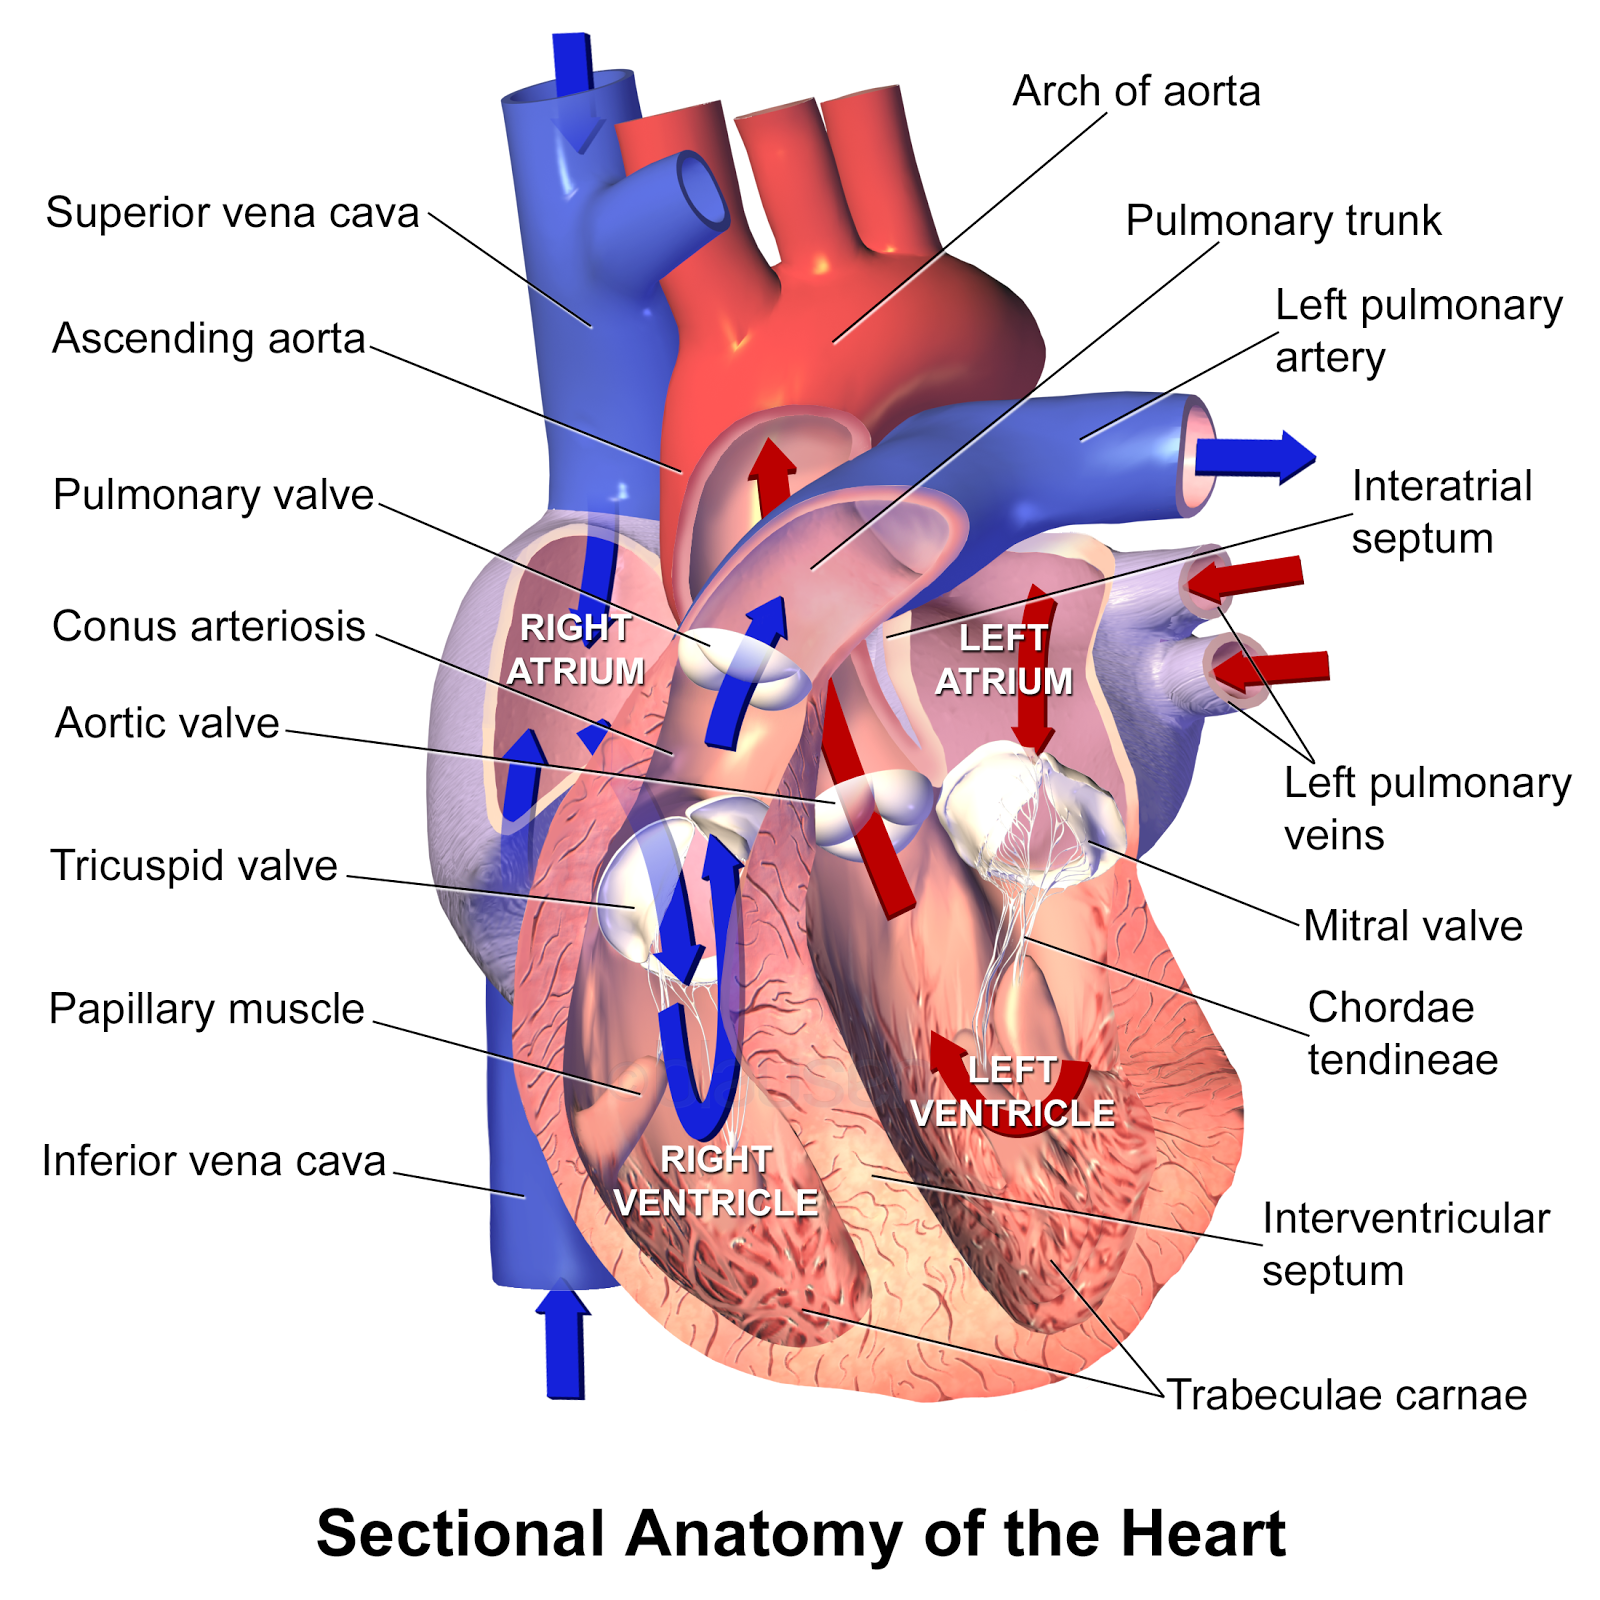
\includegraphics[width=100mm]{figures/ch2/1.png}
\caption{The human heart structure.\cite{ref1}}
\label{fig2.1}
\end{figure}

\subsection{Human heart function}
The heart circulates blood through two pathways: the pulmonary circuit and the systemic circuit.\\
In the pulmonary circuit, deoxygenated blood leaves the right ventricle of the heart via the pulmonary artery and travels to the lungs, then returns as oxygenated blood to the left atrium of the heart via the pulmonary vein.\\
In the systemic circuit, oxygenated blood leaves the body via the left ventricle to the aorta, and from there enters the arteries and capillaries where it supplies the body's tissues with oxygen. Deoxygenated blood returns via veins to the venae cavae, re-entering the heart's right atrium.\\
Of course, the heart is also a muscle, so it needs a fresh supply of oxygen and nutrients too. After the blood leaves the heart through the aortic valve, two sets of arteries bring oxygenated blood to feed the heart muscle. The left main coronary artery, on one side of the aorta, branches into the left anterior descending artery and the left circumflex artery. The right coronary artery branches out on the right side of the aorta.\\
Blockage of any of these arteries can cause a heart attack, or damage to the muscle of the heart. A heart attack is distinct from cardiac arrest, which is a sudden loss of heart function that usually occurs as a result of electrical disturbances of the heart rhythm. A heart attack can lead to cardiac arrest, but the latter can also be caused by other problems.\\
The heart contains electrical "pacemaker" cells, which cause it to contract — producing a heartbeat.\\
Each cell has the ability to be the 'band leader' and have everyone follow. In people with an irregular heartbeat, or atrial fibrillation, every cell tries to be the band leader, which causes them to beat out of sync with one another.\\
A healthy heart contraction happens in five stages:
\begin{enumerate}
	\item In the first stage (early diastole), the heart is relaxed.
	\item Then the atrium contracts (atrial systole) to push blood into the ventricle.
	\item Next, the ventricles start contracting without changing volume.
	\item Then the ventricles continue contracting while empty.
	\item Finally, the ventricles stop contracting and relax.
\end{enumerate}
Then the cycle repeats.\\
Valves prevent backflow, keeping the blood flowing in one direction through the heart.\\
\\
Some interesting data about the human heart are:
\begin{itemize}
	\item A human heart is roughly the size of a large fist.
	\item The heart weighs between about 280 to 340 grams in men and 230 to 280 grams in women.
	\item The heart beats about 100,000 times per day (about 3 billion beats in a lifetime).
	\item An adult heart beats about 60 to 80 times per minute.
	\item Newborns' hearts beat faster than adult hearts, about 70 to 190 beats per minute.
	\item The heart pumps about 6 quarts (5.7 liters) of blood throughout the body.
	\item The heart is located in the center of the chest, usually pointing slightly left
\end{itemize}
\begin{figure}[ht!]
	\centering
	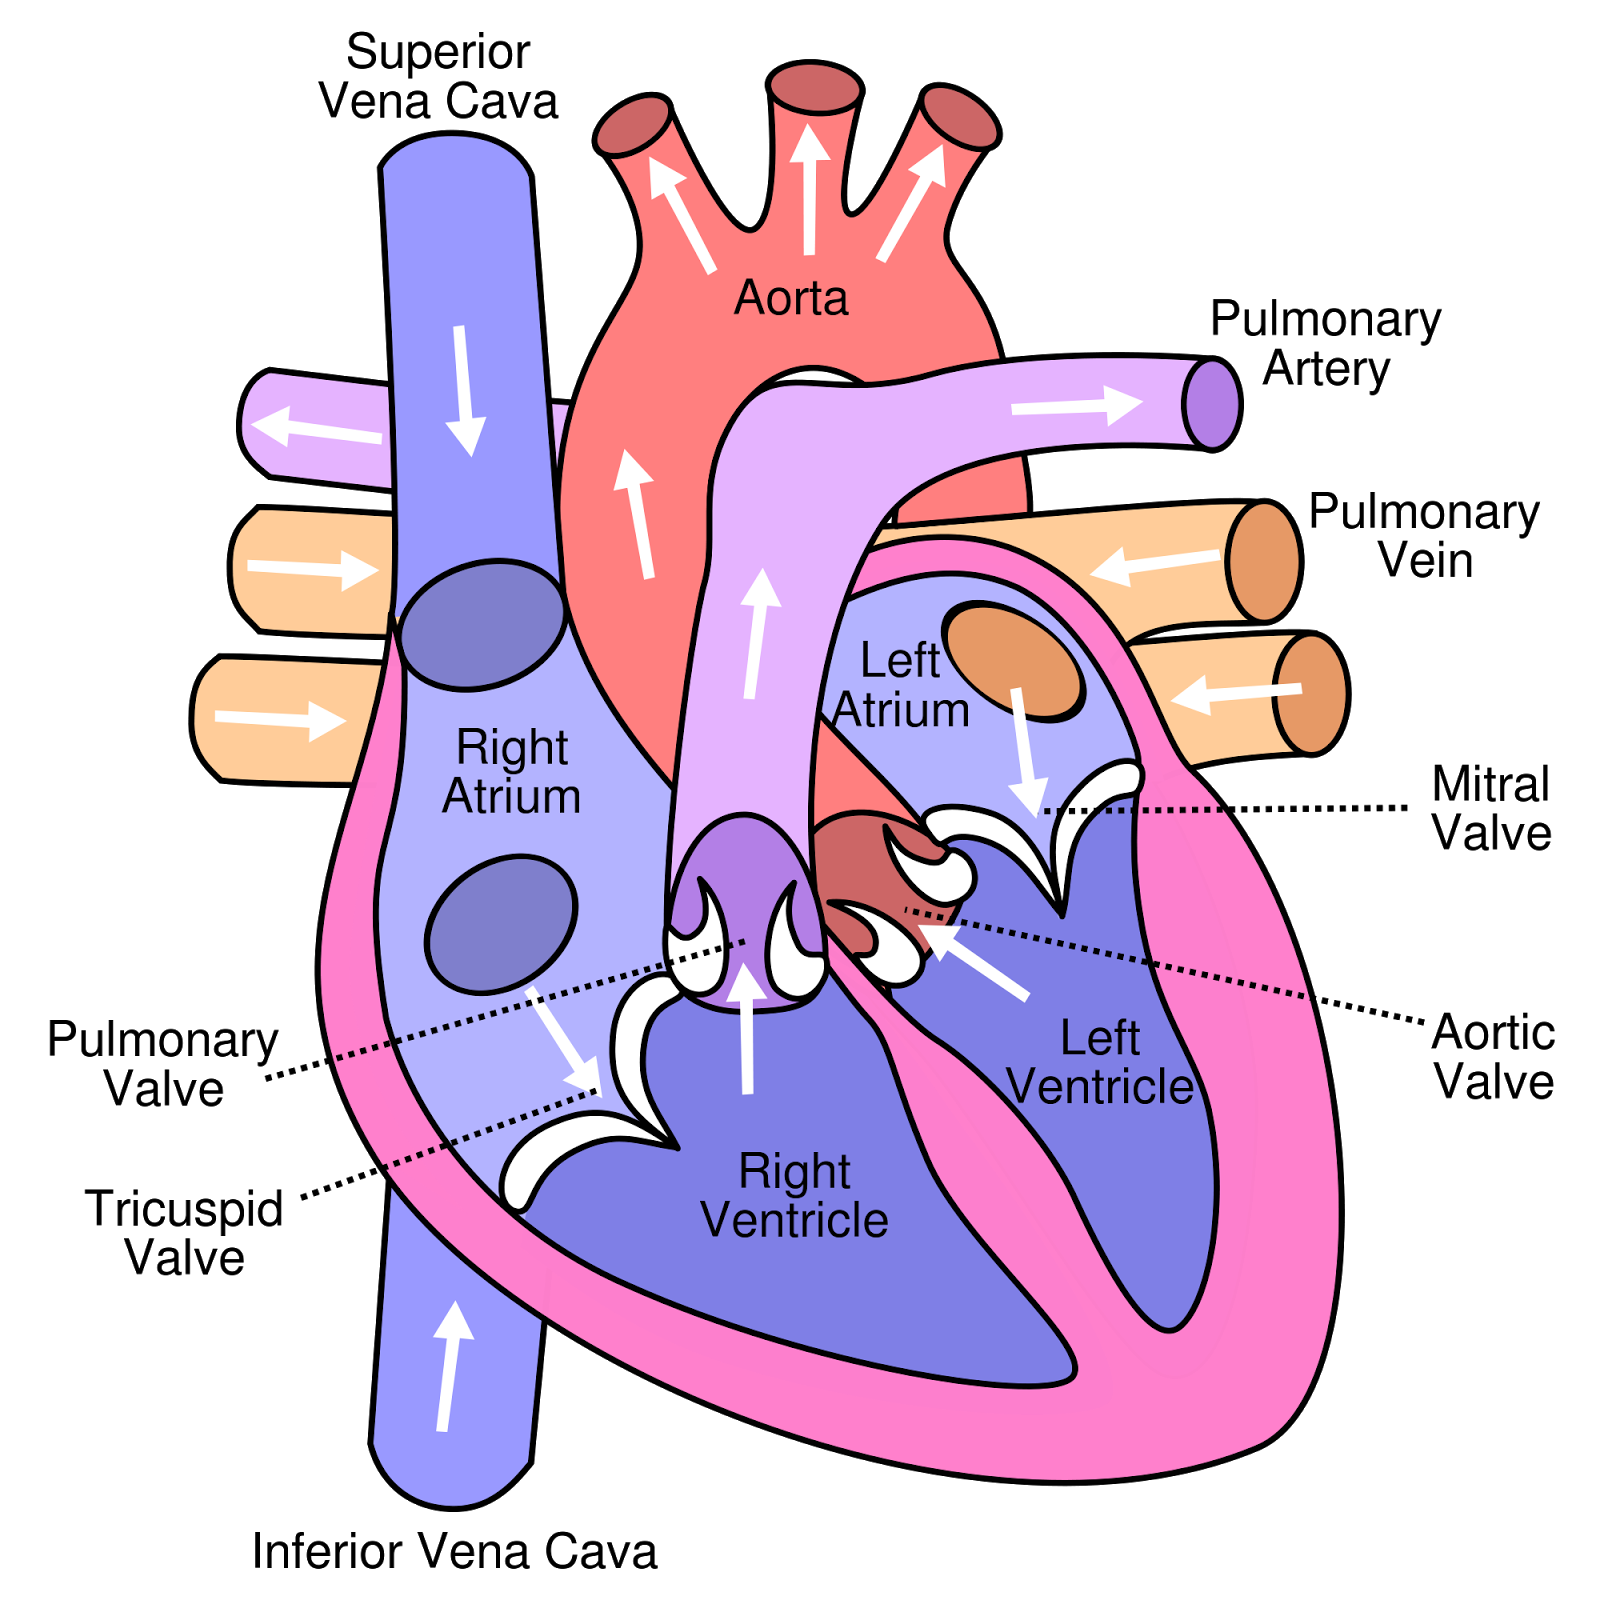
\includegraphics[width=90mm]{figures/ch2/2.png}
	\caption{The circulatory system with blood flow.}
	\label{fig2.2}
\end{figure}

\section{Heart electrical activity}
The heart has a natural pacemaker that regulates the pace or rate of the heart. It sits in the upper portion of the right atrium (RA) and is a collection of specializes electrical cells known as the SINUS or SINOATRIAL (SA) node.\\
Like the spark-plug of an automobile it generates a number of "sparks" per minute. Each "spark" travels across a specialized electrical pathway and stimulates the muscle wall of the four chambers of the heart to contract (and thus empty) in a certain sequence or pattern. The upper chambers or atria are first stimulated. This is followed by a slight delay to allow the two atria to empty. Finally, the two ventricles are electrically stimulated. In an car, the number of sparks per minute generated by a spark plug is increased when you press the gas pedal or accelerator. This revs up the motor. In case of the heart, adrenaline acts as a gas pedal and causes the sinus node to increase the number of sparks per minute, which in turn increases the heart rate. The release of adrenaline is controlled by the nervous system. The heart normally beats at around 72 times per minute and the sinus node speeds up during exertion, emotional stress, fever, etc., or whenever our body needs an extra boost of blood supply. In contrast, it slows down during rest or under the influence of certain medications. Well trained athletes also tend to have a slower heart beat.\\

\begin{figure}[ht!]
	\centering
	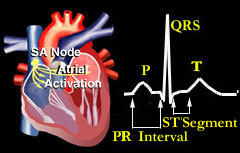
\includegraphics[width=60mm]{figures/ch2/3.png}
	\caption{The SA node fires and electrical impulses travels through the right and left atrium. \label{overflow}}
	\label{fig2.3}
\end{figure}
\begin{figure}[ht!]
	\centering
	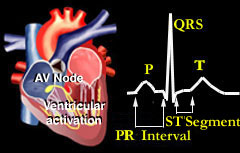
\includegraphics[width=60mm]{figures/ch2/4.png}
	\caption{The impulse then moves to the ventricular area.}
	\label{fig2.4}
\end{figure}

The sequence of electrical activity within the heart is displayed in the diagrams above and occurs as follows:
\begin{enumerate}
	\item As the SA node fires, each electrical impulse travels through the right and left atrium. This electrical activity causes the two upper chambers of the heart to contract. This electrical activity and can be recorded from the surface of the body as a "P" wave" on the patient's EKG or ECG (electrocardiogram).
	\item The electrical impulse then moves to an area known as the AV (atrio-ventricular) node. This node sits just above the ventricles. Here, the electrical impulse is held up for a brief period. This delay allows the right and left atrium to continue emptying its blood contents into the two ventricles. This delay is recorded as a "PR interval." The AV node thus acts as a "relay station" delaying stimulation of the ventricles long enough to allow the two atria to finish emptying.
	\item Following the delay, the electrical impulse travels through both ventricles (via special electrical pathways known as the right and left bundle branches). The electrically stimulated ventricles contract and blood is pumped into the pulmonary artery and aorta. This electrical activity is recorded from the surface of the body as a "QRS complex". The ventricles then recover from this electrical stimulation and generates an "ST segment" and T wave on the ECG.
\end{enumerate}

\section{Electrocardiogram}
An electrocardiogram(abbreviated as ECG or EKG) is a test that measures the electrical activity of the heartbeat. With each beat, an electrical impulse (or wave) travels through the heart. This wave causes the muscle to squeeze and pump blood from the heart. A normal heartbeat on ECG will show the timing of the top and lower chambers.\\
The right and left atria or upper chambers make the first wave called a “P wave" following a flat line when the electrical impulse goes to the bottom chambers. The right and left bottom chambers or ventricles make the next wave called a “QRS complex." The final wave or “T wave” represents electrical recovery or return to a resting state for the ventricles.\\
\begin{figure}[ht!]
	\centering
	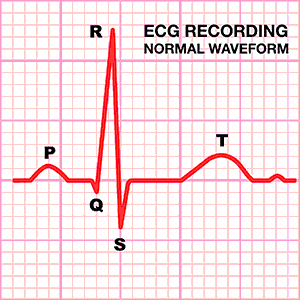
\includegraphics[width=60mm]{figures/ch2/5.png}
	\caption{An example of a normal ECG waveform. }
	\label{fig2.5}
\end{figure}
Each waves in the figure 2.5 is no other than the result of different views or perspectives of the waveforms generated from the current in the heart.\\
There are two type of ECGs recordings: the 12-lead ECG  and the rhythm strip. Both give valuable information about heart function.\\
We will focus our attention on the 12-lead ECG. It records information from 12 different views of the heart and provides a complete picture of electrical activity. The limb leads and the chest, or precordial, leads reflect information from the different planes of the heart. Different leads provide different information. The six limb leads I, II, III, augmented vector right (aVR), augmented vector left (aVL), and augmented vector foot (aVF) provide information about the heart’s frontal (vertical) plane. Leads I, II, and III require a negative and positive electrode for monitoring, which makes those leads bipolar. The augmented leads record information from one lead and are called unipolar.\\
The six precordials or V leads V1, V2, V3, V4, V5, and V6 provide information about the heart’s horizontal plane. Like the augmented leads, the precordial leads are also unipolar, requiring only a single electrode. The opposing pole of those leads is the center of the heart as calculated by the ECG.\\
The position of the leads are crucial for a right ECG recordings. It is common to use the so called Einthoven’s triangle, a set of positions to set up standard limb leads.
\begin{figure}[ht!]
	\centering
	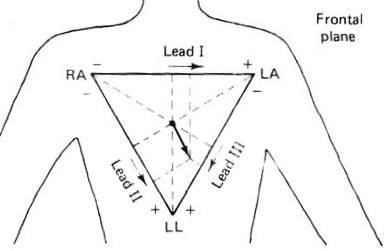
\includegraphics[width=80mm]{figures/ch2/6.png}
	\caption{The Einthoven's triangle shows the proper placement of leads over the chest.}
	\label{fig2.6}
\end{figure}
The electrodes for leads I, II, III are about equidistant from the heart and form an equilateral triangle.

\subsection{Lead I}
It provides a view of the heart that shows current moving from right to left. Because the current flows from negative to positive, the positive electrode for this lead is placed on the left arm or on the left side of the chest; the negative electrode is placed on the right arm. Lead I produces a positive deflection on ECG tracings and is helpful in monitoring atrial and hemiblock.

\subsection{Lead II}
Lead II produces a positive deflection. Place the positive electrode on the patient’s left leg and the negative electrode on the right arm. For continuous monitoring, place the electrodes on the torso for convenience, with the positive electrode below the lowest palpable rib at the left midclavicular line and the negative electrode below the right clavicle. The current travels down and to the left in this lead. Lead II tends to produce a positive, high voltage deflection, resulting in tall P, R, and T waves. This lead is commonly used for routine monitoring and is useful for detecting sinus node and atrial arrhythmias.

\subsection{Lead III}
Lead III produces a positive deflection. The positive electrode is placed on the left leg; the negative electrode, on the left arm. Along with lead II, this lead is useful for detecting changes associated with an inferior wall myocardial infarction. The axes of the three bipolar limb leads I, II, and III form a triangle around the heart and provide a frontal plane view of the heart.

\subsection{Augmented leads}
Leads aVR, aVL, and aVF are called augmented leads. They measure electrical activity between one limb and a single electrode. Lead aVR provides no specific view of the heart. Lead aVL shows electrical activity coming from the heart’s lateral wall. Lead aVF shows electrical activity coming from the heart’s inferior wall.

\subsection{Precordials leads}
The six unipolar precordial leads (V1, V2, V3, V4, V5  and V6) are placed in sequence across the chest and provide a view of the heart’s horizontal plane.
\begin{itemize}
	\item Lead V1—The precordial lead V1 electrode is placed on the right side of the sternum at the fourth intercostal rib space. This lead corresponds to the modified chest lead MCL1 and shows the P wave, QRS complex, and ST segment particularly well. It helps to distinguish between right and left ventricular ectopic beats that result from myocardial irritation or other cardiac stimulation outside the normal conduction system. Lead V1 is also useful in monitoring ventricular arrhythmias, ST-segment changes, and bundle-branch blocks.
	\item Lead V2—Lead V2 is placed at the left of the sternum at the fourth intercostal rib space.
	\item  Lead V3—Lead V3 goes between V2 and V4. Leads V1, V2, and V3 are biphasic, with both positive and negative deflections. Leads V2 and V3 can be used to detect ST-segment elevation.
	\item Lead V4—Lead V4 is placed at the fifth intercostal space at the midclavicular line and produces a biphasic waveform.
	\item Lead V5—Lead V5 is placed at the fifth intercostal space at the anterior axillary line. It produces a positive deflection on the ECG and, along with V4, can show changes in the ST segment or T wave.
	\item Lead V6—Lead V6, the last of the precordial leads, is placed level with V4 at the midaxillary line. This lead produces a positive deflection on the ECG.
\end{itemize}
\begin{figure}[ht!]
	\centering
	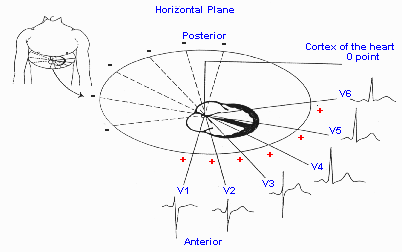
\includegraphics[width=90mm]{figures/ch2/7.png}
	\caption{Precordial leads and their position related to the heart and the chest horizontal plane.}
	\label{fig2.7}
\end{figure}

\subsection{How to read a ECG record}
Waveforms produced by the heart’s electrical current are recorded on graphed ECG paper by a stylus. An ECG paper consists of horizontal and vertical lines forming a grid. A piece of ECG paper is called an ECG strip or tracing.
\begin{figure}[ht!]
	\centering
	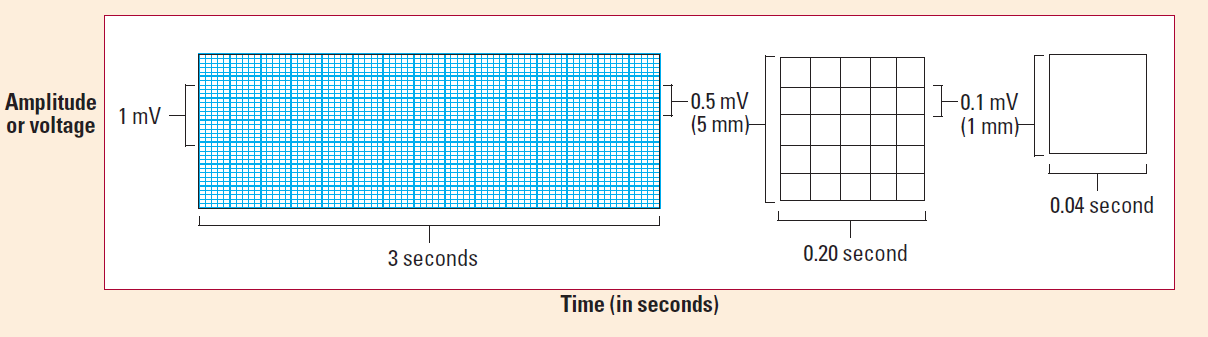
\includegraphics[width=130mm]{figures/ch2/8.png}
	\caption{A typical ECG paper.}
	\label{fig2.8}
\end{figure}
The horizontal axis of the ECG strip represents time. Each small block equals 0.04 second, and five small blocks form a large block, which equals 0.2 second. This time increment is determined by multiplying 0.04 second (for one small block) by 5, the number of small blocks that compose a large block. Five large blocks equal 1 second (5 x 0.2). When measuring or calculating a patient’s heart rate, a 6-second strip consisting of 30 large blocks is usually used. The ECG strip’s vertical axis measures amplitude in millimeters (mm) or electrical voltage in millivolts (mV). Each small block represents 1 mm or 0.1 mV; each large block, 5 mm or 0.5 mV. To determine the amplitude of a wave, segment, or interval, count the number of small blocks from the baseline to the highest or lowest point of the wave, segment, or interval.

\section{Noises and interferences}
Obtaining a reliable ECG recording is still an issue. In fact there may occur many problems interfering with the signals. Some of these problems include artifacts from patient movement and poorly placed or poorly functioning equipment.

\subsection{Artifact}
Artifact , also called waveform interference, may be seen with excessive movement (somatic tremor). The baseline of the ECG appears wavy, bumpy, or tremulous. Dry electrodes may also cause this problem to occur due to poor contact.
\begin{figure}[ht!]
	\centering
	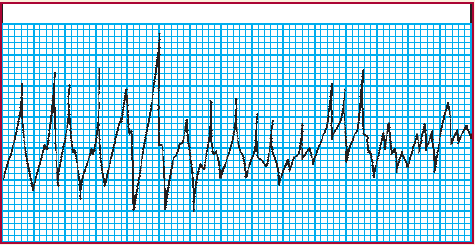
\includegraphics[width=90mm]{figures/ch2/9.png}
	\caption{ECG waveform interference due to artifact may cause monitoring to fail due to unreadable signals.}
	\label{fig2.9}
\end{figure}

\subsection{Interference}
Electrical interference, also called 60-cycle interference, is caused by electrical power leakage. It may occur due to interference from other room equipment or improperly grounded equipment. As a result, the lost current pulses at a rate of 60 cycles per second. This interference appears on the ECGs as a baseline that is thick and unreadable.
\begin{figure}[ht!]
	\centering
	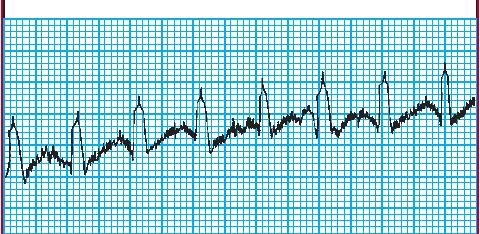
\includegraphics[width=90mm]{figures/ch2/10.png}
	\caption{Electrical interference causes the baseline to be unstable and the signal is corrupted.}
	\label{fig2.10}
\end{figure}

\subsection{Wandering baseline}
A wandering baseline undulates, meaning that all waveforms are present but the baseline is not stationary.  It can be caused by movement if the chest wall during respiration, poor electrode placement, or poor electrode contact.
\begin{figure}[ht!]
	\centering
	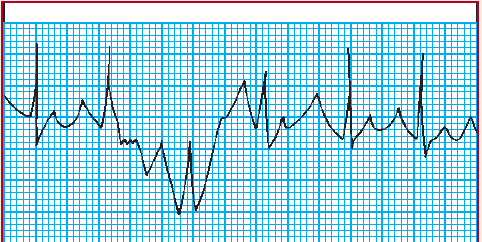
\includegraphics[width=90mm]{figures/ch2/11.png}
	\caption{An example of baseline wandering due to artifacts.}
	\label{fig2.11}
\end{figure}

\subsection{Faulty equipment}
Faulty equipment, such a s broken lead wires and cables, can also cause monitoring problems.